\chapter{Konzeption}\label{ch:Konzeption}

In diesem Kapitel werde ich die Konzeption der Thesis beschreiben und einige wichtige Algorithmen näher erläutern. Generell beruht die Konzeption dieser Thesis auf dem ROS~(Robot Operating System)-Framework, welches quelloffen unter der BSD-Lizenz zur Verfügung steht~\footnote{\url{http://www.ros.org/is-ros-for-me/}}.

\section{Generelles zur Konzeption}
Die Konzeption besteht aus iterativen Schritten in denen ein bestimmtes Verhalten erarbeitet und anschließend ausgewertet wird. Dabei wird nicht mit dem erstbesten Ergebnis weiter gemacht, sondern es werden verschiedene Herangehensweisen getestet und für die nächsten Schritte evaluiert. Auch viele Iterationen später könnte sich ein Vorgehen, welches zunächst als unzureichend eingestuft wurde, als das bessere herausstellen.\\

Die Konzeption findet auf Ubuntu LTS 16.04 mit der ROS-Version 'Lunar' statt, da diese beiden Komponenten das derzeit stabilste Duo bilden. Aufgrund mangelnder Kapazitäten, befindet sich das Ubuntu-System in einer Virtuellen Maschine, was, bis auf einen höheren Ressourcen-Verbrauch, allerdings keinerlei erkennbare Nachteile mit sich zieht.

Da ein experimentelles Vorgehen direkt an realen Robotern zu Aufwändig wäre, insbesondere was die Zeitkosten für die Durchführung einer Simulation angeht, beruht die Konzeption auf der Node Turtlesim~\footnote{\url{http://wiki.ros.org/turtlesim}} von ROS~(siehe~\autoref{subsec:Grundlagen_Turtlesim}). Die Turtlesim wurde dahingehend angepasst, dass die Bilder der Turtles durch wesentlich kleinere Bilder schwarzer Pfeile ersetzt wurden. Diese bieten mehr Platz und übersichtlichkeit. Das Verhalten der Turtles selbst in der Simulation ist unverändert.
Generell ist die Turtlesim nicht dafür gemacht worden aufwändigere Simulationen zu erproben, weswegen nicht alles visuell dargestellt werden konnte und vieles aus den Daten herausgelesen werden muss die gesammelt wurden.

\section{Nachbau des Schwarms nach Craig Reynolds}
Da der Transport der Schwarms auf den 3 (bzw. 4) Grundregeln des Schwarmverhaltens besteht welche von Craig Reynolds erstmals modelliert wurden (\note{http://www.red3d.com/cwr/boids/}) galt es diese zunächst nachzustellen und zu analysieren. Der Schwarm wurde zunächst nachgebaut ohne auf die spätere Verwendung für Transporte zu achten, da diese (möglichst) ohne Kompromisse auf dem Schwarm-Prinzip aufbauen.

Die Roboter haben durch ROS sehr viele Informationen über die anderen Roboter. Jede Einheit kennt die genaue Position der anderen Roboter und deren Ausrichtung. Diese Informationen werden bei jeder Bewegung an die anderen Roboter (und sich selbst) gesendet und über Callback-Funktionen in einem Array gespeichert. Diese Funktion ist bereits von der Turtlesim bereitgestellt und wird in der späteren Implementierung von einem Modul ersetzt werden müssen dass die eigene Position möglichst genau ermittelt und den anderen mitteilt. Der modulare aufbau des Systems macht es ohne weitere Probleme möglich solche Module auszutauschen.

Um die Roboter eindeutig identifizieren zu können wird ihnen bei Programmstart eine eindeutige ID zugewiesen. Durch diese können Nachrichten eindeutig ihrem Ursprung zugeordnet werden, was das Updaten der jeweiligen Positionsdaten erst möglich macht.

\subsection*{Messages}
Da die Roboter in der Simulation keine Sensoren haben um die Position oder Ausrichtung ihrer Nachbarn zu erkennen, sind sie darauf angewiesen dass die Roboter selbst ihre Daten mit den anderen Teilen. In ROS funktioniert dies über einen ROS-Master der im Sinne des Subscriber-Publisher-Prinzips Messages zu einem bestimmten Topic entgegen nimmt und sie an diejenigen weiterverteilt die das entsprechende Topic abonniert haben. Der ROS-Master ist dabei zwar eine zentrale Einheit, kann aber auf dem System eines Roboters untergebracht werden. Es ist also keine weitere Einheit notwendig, wodurch das Gesamt-System homogener bleibt, wenn auch immer eine direkte Verbindung zum Master bestehen bleiben muss.

Für eine einfache Schwarm-Simulation, ist nur eine Art von Nachricht notwendig. Diese enthält die Position und Ausrichtung der Roboter und wird nach jedem ausgeführten Bewegungs-Befehl gesendet. Um das System der Roboter einfacher zu halten abonnieren die Roboter auch die Bewegungs-Daten von sich selbst. Dadurch ist es nicht notwendig diese gesondert zu behalten, sondern die Daten werden in das eigene System eingepflegt, wie die von allen anderen Einheiten auch. Möchte ein Roboter dann auf die eigenen Daten zugreifen, kennt er seinen Index und greift auf die Daten normal zu.

\subsection*{System-Takt: Ticks}
Der Ablauf eines Programms geschieht in Ticks (der Takt des Systems, periodische Zeitabstände) in denen zuerst eine Aktion gestartet und danach eine kurze Zeit gewartet wird um Nachrichten anderer Roboter zu empfangen und zu verarbeiten. Es ist damit impliziert nur eine Bewegungs-Aktion pro Tick möglich. Diese kann allerdings Drehung und Fahren kombinieren.
Die Bewegung einer Turtle wird von ROS genau 1 Sekunde lang ausgeführt, die Steuerung der bewegten Entfernung pro Tick lässt sich daher nur über die Geschwindigkeit der Bewegung steuern. In der Praxis hat sich aufgrund von weiteren Verzögerungen in der Turtlesim eine Tick-Länge von 1.1 Sekunden bewährt.

Entschließt sich ein Roboter dazu sich nicht zu bewegen, muss er einen 'leeren' Bewegungsbefehl senden der dazu führt dass sich der Roboter nicht bewegt und somit einen Tick abschließen, statt einfach zu warten und nichts zu senden. Der Grund hierführ liegt darin, dass die Systeme Single-Thread Architekturen sind und das Abfragen der Topics expliziert ausgelöst werden muss. Dies geschieht über eine Funktion in ROS die aufgerufen wird und die automatisch alle abonnierten Topics abfragt um dann die entsprechenden Callback-Funktionen auszuführen. Außerdem werden dadurch die eigenen Daten auf den Robotern aufgefrischt und eventuelle Informationen gesendet die nichts mit der Bewegung zu tun haben. Das abschließen eines Ticks synchronisiert damit generell die Daten des eigenen Systems mit dem der anderen.

\subsection*{Einhalten der 4 Grundregeln}
Die Roboter wurden als autonome Einheiten konzipiert die sich ausschließlich anhand von 3 fixen Parametern bewegen und dabei versuchen die 4 Grundlegen des Schwarmverhalten einzuhalten.

\subsubsection*{Ausrichtung: Passe deine Bewegungsrichtung deinen Nachbarn an}

\begin{wrapfigure}{r}{\pictureWidth}
	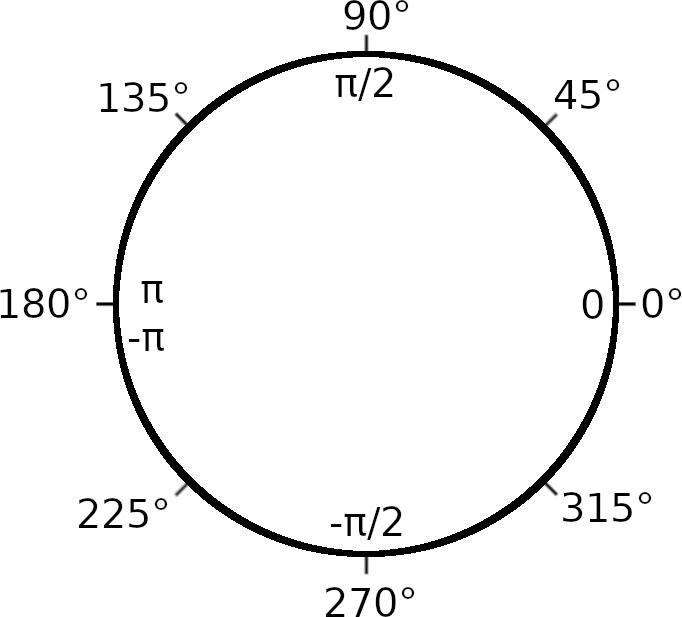
\includegraphics[width=\pictureWidth,keepaspectratio]{graphics/WinkelTemplate.png}
	\caption{Winkel-Übersicht}
	\label{pic:WinkelUebersicht}
\end{wrapfigure}

Da ein Roboter die Position und Ausrichtung jedes anderen Roboters kennt ist es ohne weiteres möglich die durchschnittliche Ausrichtung der Nachbarschaft zu ermitteln. Dafür wird zunächst jeder Roboter aussortiert der nicht nahe genug ist um zur Nachbarschaft zu zählen. Der einfache Durchschnitt über die Summe mehrerer Winkel würde jedoch zu einem mathematischen Schnitt führen, statt zu einem der in der Praxis relevant ist. Daher müssen die Winkel für die Berechnung zunächst in Vektoren umgerechnet werden. Diese Vektoren werden dann addiert und der resultierende Gesamtvektor wird wieder in einen Winkel zurück gerechnet.

In~\autoref{pic:WinkelUebersicht} ist eine Übersicht über die Winkel zu sehen wie sie im System genutzt werden. ROS selbst arbeitet mit dem Bereich von [-3.14, 3.14] wohingegen die Steuerung der Roboter mit dem Bereich [0°, 360°] arbeitet, da dieser besser bearbeitet (und von Menschen gelesen) werden kann. Vor dem Senden eines Bewegungs-Befehls wird der Winkel automatisch so umberechnet dass ROS ihn akzeptiert. Wird ROS ein zu großer Winkel gesendet, z.B.: 400, so wird sich der Roboter einfach sehr schnell drehen, sonst aber keine weiteren Fehler produzieren.
 
\subsubsection*{Zusammenhang: Versuche deinen Nachbarn nahe zu sein}

\begin{wrapfigure}{r}{\pictureWidth}
	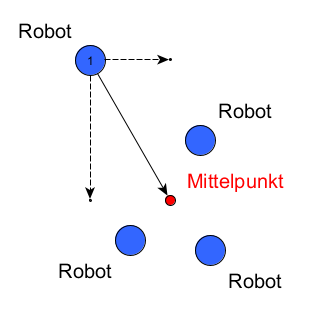
\includegraphics[width=\pictureWidth,keepaspectratio]{graphics/SchwarmMittelpunktBerechnung.png}
	\caption{Berechnung des Mittelpunkts}
	\label{pic:BerechnungMittelpunkt}
\end{wrapfigure}

Dieser Abschnitt wird realisiert indem ebenfalls zuerst die Roboter aussortiert werden die nicht nahe genug sind um zur Nachbarschaft zu gehören. Anschließend wird ein simpler Durschnitt über alle Positionen (x/y - Koordinaten) der vorhandenen Roboter berechnet. Die resultierenden Koordinaten werden von den eigenen Koordinaten abgezogen um die relative Position des Schwarm-Mittelpunkts zu bekommen. Indem man nun die relativen Koordinaten als Vektor behandelt und dadurch zu einem Winkel umrechnet, erhält man letztlich den relativen Winkel den der Mittelpunkt der Nachbarschaft zum Roboter hat.

\paragraph*{Beispiel für eine fehlerhafte Winkel-Berechnung}
Zwei Roboter mit den Winkeln 45° und 315° würden zu einem durchschnittlichen Winkel von 180° führen. Der richtige Winkel in Anbetracht der Ausrichtung wäre jedoch 0°.\\

Dabei ist der Mittelpunkt der Nachbarschaft wie er in~\autoref{pic:BerechnungMittelpunkt} zu sehen ist allerdings nicht zwingend der Mittelpunkt der konvexen Hülle die die Nachbarschaft umgrenzt. Mehrere Roboter ziehen den Mittelpunkt der Nachbarschaft mehr in ihre Richtung. Der Vorteil dieser Methode ist, dass die Wahrscheinlichkeit höher ist einzelne Roboter zu verlieren, statt ganzer Gruppen.

\subsubsection*{Abschottung: Vermeide Kollisionen mit deinen Nachbarn}

\begin{wrapfigure}{r}{\pictureWidth}
	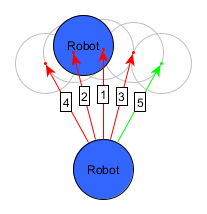
\includegraphics[width=\pictureWidth,keepaspectratio]{graphics/AusweichenAlgorithmus.png}
	\caption{Ausweichen gegenüber Hindernissen}
	\label{pic:AusweichenAlgorithmus}
\end{wrapfigure}

Damit die Roboter nicht beschädigt werden haben sie eine Größe erhalten und prüfen ihre Position mit der der anderen ab. Eine Bewegung wird als gültig befunden, wenn der Roboter an seinem Zielpunkt mindestens seine Größe als Abstand zu allen anderen Robotern hat. Praktisch wurde die Größe mit um 10\per erweitert um eine gewisse Sicherheit zu gewährleisten.

\paragraph*{Unzureichende Erkennung auf dem Weg}
Um die Berechnung einfacher zu gestalten und Ressourcen zu schonen wurde nicht der Weg selbst überprüft. Es ist also möglich, dass ein Roboter weder auf seinem Ursprungs- oder Zielort mit anderen Robotern kollidiert, wohl aber auf dem Weg dorthin. Ebenfalls ist es in der Turtlesim nicht möglich eine angefangene Bewegung wieder abzubrechen. Kommt es also während der Ausführung zu einer Kollision, z.B. weil sich zwei Roboter auf einander zubewegen, kann diese nicht mehr verhindert werden. Ein Ausgleich in der Simulation ist eine Abfrage ob sich zwei Roboter "ineinander" befinden. Die entsprechenden Roboter werden dann auf direkter Luftlinie voneinander weggeschoben um wieder einen plausiblen physikalischen Zustand einzunehmen.
Im der Praxis sollte eine Kollision auf dem Weg kein Problem darstellen. Zum einen lassen sich mit Sensoren und nebenläufigen Routinen auch Positionen zwischen zwei Ticks feststellen, zum anderen kann die Frequenz der Ticks wesentlich schneller eingestellt werden, sodass sich die Roboter effektiv nur wenige Millimeter pro Tick bewegen, dafür mit über 100 Ticks pro Sekunde. Letztlich kommt es auf die Leistung des verwendeten Computers an.


Findet eine Kollision statt, prüft der Roboter Ausweichmöglichkeiten. Der Algorithmus wird dabei angewendet, egal ob das Hinderniss ein anderer Roboter ist oder eine Gefahrenzone. Ist der gerade Weg nicht möglich wird abwechselnd versucht nach links und rechts auszuweichen, wie in~\autoref{pic:AusweichenAlgorithmus} gezeigt wird. Dabei wird der Winkel der zum Ausweichen genutzt wird stufenweise erhöht, bis man letztlich 180° zu beiden Seiten erreicht, was einem Schritt rückwärts entspricht. Führt auch dieser letzte Winkel nicht zu einem erfolgreichen Ergebnis, wird ein Tick abgewartet, die Position der anderen Roboter aktualisiert und der Algorithmus startet mit einer leicht geringeren Geschwindigkeit (was ebenfalls einer leicht geringeren Bewegungsdistanz entspricht) erneut.

All diese Bewegungen sind interne Simulationen die keinerlei physische Reaktionen erzeugen. Erst wenn eine Simulation eine erfolgreiche Bewegung generieren konnte wird diese auch ausgeführt.

\subsubsection*{Flucht: Fliehe vor Dingen, die eine potentielle Gefahr darstellen}

Gefahren wie Hindernisse, Löcher im Boden oder Zonen mit sich bewegenden Maschinen können die Roboter beschädigen, weshalb es gilt diesen Auszuweichen. Im System werden Hindernisse global in einem Container gespeichert. Bei jeder Bewegung wird überprüft ob man mit der angestrebten Bewegung eine Gefahrenzone betreten würde und wenn ja, wird, wie im vorigen Abschnitt erläutert, versucht auszuweichen.

Gefahrenzonen sind dabei Objekte die sich aus verschiedenen Geometrien zusammensetzen. Bisher sind Quader und Kreise umgesetzt. Diese Geometrien können mit verschiedenen Positionen angegeben werden, nicht zwangsweise zusammenhängend. Bewegt sich ein Objekt an einen absoluten oder relativen Ort, bewegen sich alle gespeicherten Geometrien ebenfalls, sodass der Zustand konsistent bleibt.

Gespeicherte Objekte haben eine eindeutige ID die es erlaubt ihnen über globale Broadcasts ein Update der Position zu geben. Dadurch können Hindernisse in Echtzeit beobachtet, die gesammelten Informationen geteilt und von den einzelnen Robotern auch genutzt werden.

\subsection*{Parameter der Bewegung}

Konfiguriert wird das Schwarmverhalten der Roboter durch 4 Parameter, die in den nachfolgenden Abschnitten näher erläutert werden.

\paragraph*{Geschwindigkeit} Gibt an wie schnell ein Roboter sich bewegt. Da eine Bewegung immer genau 1 Sekunde lang ausgeführt wird, gibt dieser Wert auch direkt die Bewegungs-Distanz an. Ein kleinerer Wert sorgt für langsamere, aber auch "vorsichtigere" Roboter. Optimal wäre ein kleiner Wert in Geschwindigkeit aber eine hohe Frequenz der Ticks.

\paragraph*{Lokale Reichweite} Da ein Roboter nur seine unmittelbare Umgebung imitiert braucht es dafür einen Grenzwert. In dieser Thesis wurde sich für eine Begrenzung in der Reichweite (im Gegensazu zu einer Begrenzung in der Anzahl der Roboter) entschieden. Einheiten die weiter weg sind als dieser Wert (in der entsprechenden Maßeinheit) werden für Berechnungen ignoriert. Ein Wert kleiner als die eigene physikalische Größe führt zwangsläufig dazu, dass der Roboter nur sich selbst beachtet.

\paragraph*{Freier Wille} Einheiten im Schwarm orientieren sich nicht nur an seinen Nachbarn, sondern haben auch in gewisser Weise einen eigenen Willen. Nachdem die Berechnung der Orientierung am Schwarm abgeschlossen ist wird der eigene Wille einberechnet. Das ist ein Winkel der zufällig zwischen [-x/2, x/2] ausgesucht wird und dem bisherigen Winkel aufgerechnet wird.

\paragraph*{Nähe zum Schwarm} Dieser Wert ist verbunden mit der Regel "Zusammenhang: Versuche deinen Nachbarn Nahe zu sein". Ein Roboter hat den Drang seinem Schwarm nahe zu bleiben und versucht sich bis zu einem gewissen Grad in dessen Richtung zu bewegen. Wie später in der Analyse hervorgehen wird, muss dieser Wert vorsichtig gewählt werden, da bereits ein recht geringer Wert dazu führt dass die Bewegung diesem Parameter große Priorität gewährt.\\

\begin{wrapfigure}{r}{\pictureWidth}
	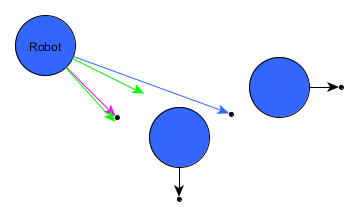
\includegraphics[width=\pictureWidth,keepaspectratio]{graphics/BerechnungBewegung.png}
	\caption{Berechnung einer Bewegung}
	\label{pic:BerechnungBewegung}
\end{wrapfigure}

In~\autoref{pic:BerechnungBewegung} ist die Berechnung einer Bewegung skizziert. Die Pfeile geben dabei nur Richtungen an und sind nicht als Vektoren zu verstehen, die eine Aussage über die bewegte Entfernung treffen.

Der pinke Pfeil ist das Resultat der Berechnung des Mittelwerts der Winkel den die anderen Roboter in ihrer letzten Bewegung eingenommen haben.

Der blaue Pfeil ist der Mittelpunkt des Schwarms (in diesem Fall sind beide Roboter ein Teil der Nachbarschaft) auf den der Roboter sich aufgrund seiner Gruppenzugehörigkeit zubewegen möchte.

Die beiden grünen Pfeile sind letztlich die obere und untere Grenze des Spielraums den der Roboter durch seinen freien Willen bekommt, welcher durch die Ausrichtung zum Schwarm-Mittelpunkt leicht verschoben wurde. Ein zufälliger Winkel wird letztlich aus diesen Grenzen entnommen und anschließend auf Gültigkeit (keine Kollisionen) getestet um dann ausgeführt zu werden.

\subsection*{Analyse}

\begin{wrapfigure}{r}{\pictureWidth}
	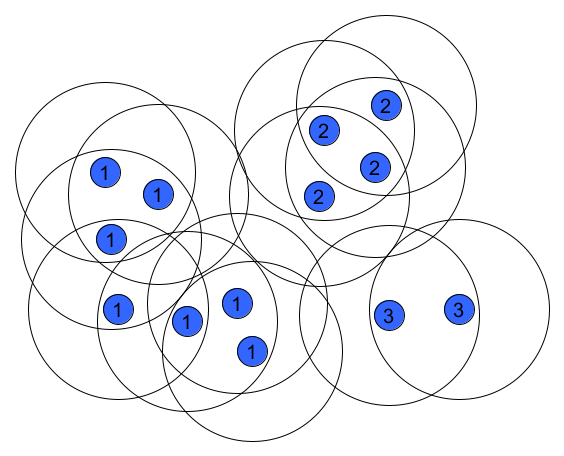
\includegraphics[width=\pictureWidth,keepaspectratio]{graphics/SchwarmEinordnung.png}
	\caption{Einordnung der Roboter in Schwärme}
	\label{pic:SchwarmEinordnung}
\end{wrapfigure}

Nachdem die Implementierung des Schwarms abgeschlossen ist galt es diese zu testen und Statistiken zu erheben. Dazu wurde die Simulation mit verschiedenen Parametern gestartet und 25 Roboter zufällig in der Simulation verteilt. Die Simulationen wurden für 1 Stunde laufen gelassen und in 10s-Abständen gemessen wie viele Schwärme sich gebildet haben.
Ein Schwarm war hierbei eine zusammenhängende Kette von Robotern die nicht weiter als ihre lokale Reichweite voneinander entfernt sind. Das bedeutet, dass alle Roboter innerhalb eines Schwarm die anderen beeinflusst. Teilweise mag dies direkt geschehen sein, wenn sie innerhalb der lokalen Reichweite waren, aber auch indirekt ist es möglich, indem Roboter beeinflusst wurden, durch Roboter die von anderen beeinflusst wurden. \autoref{pic:SchwarmEinordnung} zeigt ein Beispiel mit 2 Schwärmen. Die Roboter sind als blaue Kreise eingezeichnet, ihre jeweilige lokale Reichweite als schwarzer Kreis drum herum.
Da das Verhalten der Roboter aufgrund ihres freien Willens und der zufälligen Platzierung in der Simulation starken Schwankungen ausgesetzt ist, wurden immer 10 Simulationen gestartet und aus den mittleren 6 Werten ein Durchschnitt gebildet. Dadurch wurden Ausreißer eliminiert und die Statistiken können sinnvolle Mittelwerte zeigen. Der Rand der Simulation wurde als Hinderniss gewertet, bedeutet dass die Roboter nicht stumpf weiter gefahren sind nachdem dieser erreicht wurde, sondern sie versucht haben diesem auszuweichen.

Bei 3 Parameter und teilweise über 5 Möglichkeiten diese Einzustellen ergäbe sich eine Anzahl an Simulationen die zeitlich nicht machbar ist und deren Vorstellung aufgrund zu kleiner Unterschiede nicht lohnenswert ist. Es werden daher nur ausgewählte Ergebnisse vorgestellt.

\subsubsection*{Statistik: Freier Wille}\label{subsubsec:StatistikFreierWille}

\begin{figure}
	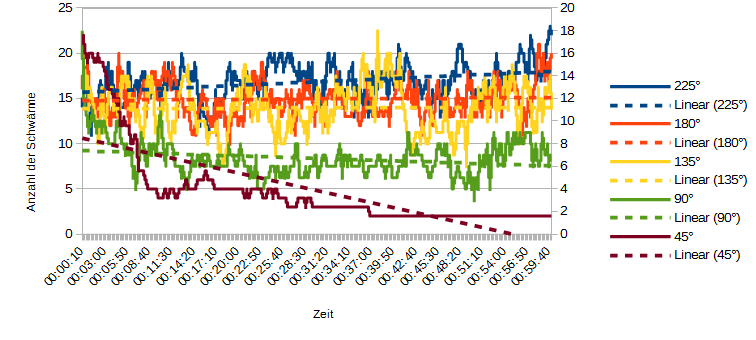
\includegraphics[width=\textwidth,height=\statisticHeight]{graphics/Statistics/FlockGeneral/LocalRange1Speed01ToFlock0.png}
	\caption{Entwicklung der Schwärme in Abhängigkeit ihres freien Willens}
	\label{pic:GeneralFlockStatistic1}
\end{figure}

In~\autoref{pic:GeneralFlockStatistic1} zu sehen, ist eine Statistik die die Entwicklung von Schwärmen mit verändertem freien Willen zeigt.

\paragraph*{Eigenschaften des Schwarms:}
\begin{itemize}
	\item Größe des Schwarms: 25 Roboter
	\item Lokale Reichweite: 5\per der Größe der Simulation
	\item Geschwindigkeit: 10\per der lokalen Reichweite
	\item Drang zur Gruppierung: 0\per
	\item Freier Wille: Variabel
\end{itemize}

\begin{wrapfigure}{r}{\pictureWidth}
	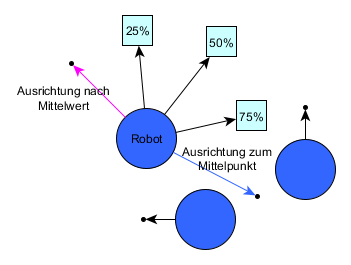
\includegraphics[width=\pictureWidth,keepaspectratio]{graphics/BerechnungDrangZurGruppe.png}
	\caption{Berechnung des Drangs zur Gruppierung}
	\label{pic:BerechnungDrangZurGruppe}
\end{wrapfigure}

Wie genau der Drang zur Gruppierung in Prozente eingeteilt ist, wird in \autoref{pic:BerechnungDrangZurGruppe} skizziert dargestellt.

Über die X-Achse hinweg ist die Zeit der Simulation von 0-60 Minuten, die Y-Achse zeigt die Anzahl der vorhandenen Schwärme nach obiger Definition. Grundsätzlich wäre es innerhalb der Simulation aufgrund des verfügbaren Platzes möglich gewesen, dass jeder Roboter nur sich selbst als Schwarm hat.
Neben den Graphen selbst die die Entwicklung der Schwärme zeigen, ist ebenfalls ein linearer Trend eingezeichnet worden, der in gleicher Farbe und gestrichelter Linie eingezeichnet ist.

Zu sehen ist, dass ein Roboter mit einem freien Willen von 225° (112.5° in beide Richtungen) eher dazu neigt sich zu verteilen statt sich zu sammeln. Der Einfluss der Regel sich nach seinen Nachbarn auszurichten liegt bei unter 50\per und unterliegt somit dem freien Willen. Dass es dennoch dazu kam dass sich Schwärme gebildet haben, resultiert einerseits daraus, dass aus der Menge [-112.5°, 112.5°] der letztliche Wert zufällig ermittelt wurde, der Durchschnitt also um 0° herum liegt, mit einer durchschnittlichen Abweichung von 56.25° zu beiden Seiten. Anderseits spielt aber auch der mangelde Platz zum verteilen eine Rolle und Roboter die zufällig aufeinander zugefahren sind im nächsten Tick als Schwarm erkannt wurden, unabhängig vom Grund warum sie zusammen waren.

Bei einem freien Willen von 180° und 135° zeigt sich der Trend nahezu konstant. Schwärme wurden gebildet und im gleichen Maße wieder aufgelöst.

Ab einem freien Willen von 90° und darunter zeigt sich dagegen ein Trend zur Gruppierung. Der Drang zur Gruppierung nimmt einen Großteil des Verhaltens ein und auf lange Sicht wäre die Zahl der Schwärme gegen 1 gesunken. Dies zeigt sich vor allem bei einem Wert von 45°, der bereits während einiger der einstündigen Simulationen dazu geführt hat, dass sich alle Roboter zu einem einzigen Schwarm versammelt haben.

\subsubsection*{Statistik: Gruppierungsdrang}

\begin{figure}
	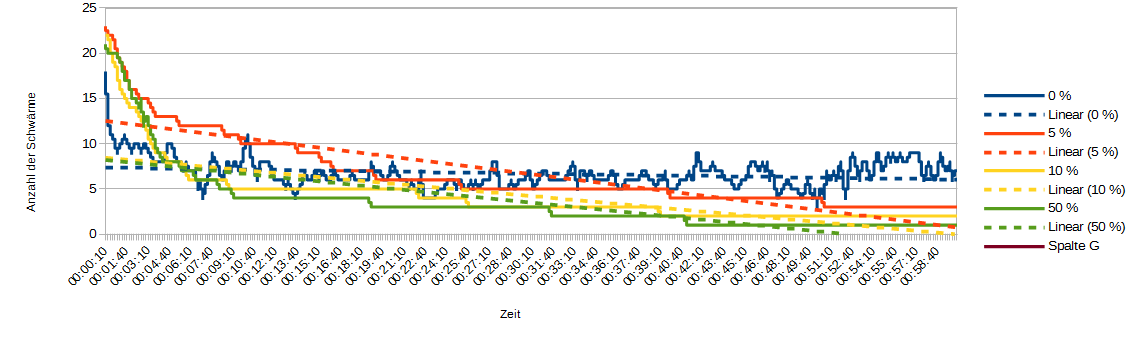
\includegraphics[width=\textwidth, height=\statisticHeight]{graphics/Statistics/FlockGeneral/LocalRange1Speed01FreeWill90.png}
	\caption{Entwicklung der Schwärme in Abhängigkeit ihres Dranges zur Gruppierung mit 90° eigenem Willen}
	\label{pic:GeneralFlockStatistic2}
\end{figure}

In~\autoref{pic:GeneralFlockStatistic2} und~\autoref{pic:GeneralFlockStatistic3} zu sehen, sind Statistiken die die Entwicklung von Schwärmen mit verändertem Drang zur Gruppierung zeigen. Über die X-Achse hinweg ist die Zeit der Simulation von 0-60 Minuten, die Y-Achse zeigt die Anzahl der vorhandenen Schwärme. In der ersten Statistik behielten sie dabei einen freien Willen von 90°, bei der zweiten wurde ein freier Wille von 225° eingestellt.

\paragraph*{Eigenschaften des Schwarms:}
\begin{itemize}
	\item Größe des Schwarms: 25 Roboter
	\item Lokale Reichweite: 5\per der Größe der Simulation
	\item Geschwindigkeit: 10\per der lokalen Reichweite
	\item Freier Wille: 90° bzw. 225°
	\item Drang zur Gruppierung: Variabel
\end{itemize}

Bei einem freien Willen von 90° ist zu sehen, dass die Anzahl der Schwärme bei einem Drang zur Gruppierung von 0\per konstant bleibt. Diese Entwicklung war bereits in \autoref{subsubsec:StatistikFreierWille} zu sehen. Die Start-Anzahl war dabei in allen Simulationen annähern gleich.
Sobald der Drang zur Gruppierung über 0\per steigt, zeigt sich, dass die Roboter sich abhängig vom eingestellten Wert unterschiedlich schnell zu Schwärmen zusammenziehen und diese auch nicht wieder verlassen. Ein höherer Wert sorgte dabei analog dafür, dass sich die Schwärme schneller sammelten.

\begin{figure}
	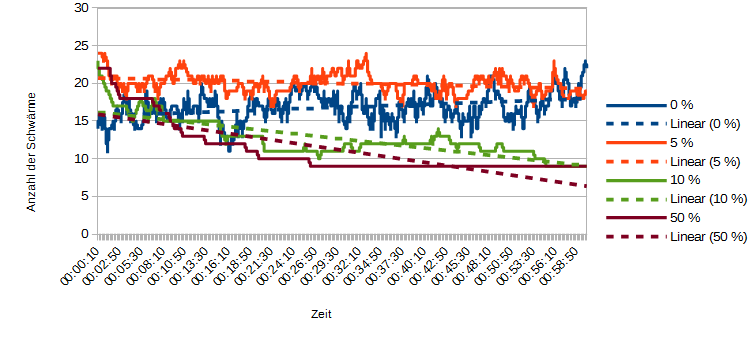
\includegraphics[width=\textwidth, height=\statisticHeight]{graphics/Statistics/FlockGeneral/LocalRange1Speed01FreeWill225.png}
	\caption{Entwicklung der Schwärme in Abhängigkeit ihres Dranges zur Gruppierung mit 225° eigenem Willen}
	\label{pic:GeneralFlockStatistic3}
\end{figure}

Bei einem freien Willen von 225° zeigt sich dagegen deutlich mehr Varianz. Die Entwicklung um 0\per herum ist dabei wieder die gleiche wie in \autoref{subsubsec:StatistikFreierWille} bereits zu sehen war. Ein Wert von 5\per neigt die Trendlinie zwar leicht nach unten, die Daten zeigen aber nach wie vor hohe Fluktuationen und Schwärme die sich zunächst gebildet haben, brechen aufgrund des großen freien Willens wieder auseinander und die Roboter trennen sich. Bei 10\per wird der Trend zwar umso deutlicher, die Fluktuationen sind aber nach wie vor zu sehen und Schwärme neigen noch immer dazu sich gelegentlich zu trennen. Erst ab einem Wert von 50\per bleiben Schwärme stabil und langsam aber sicher fügen sich alle Roboter zu einem einzelnen Schwarm zusammen.

\subsubsection*{Statistik: Negativer Gruppierungsdrang}

Zum Schluss wurde noch eine Statistik mit negativem Gruppierungsdrang erstellt. Hintergrund dieses Versuchs war es, Roboter verteilen zu lassen. Damit sie sich während des Leerlaufs nicht versammeln und so in ihrer Masse zu einem größeren Hinderniss werden, wurde versucht die Roboter dazu zu bringen sich zu meiden und damit auszulösen dass sie sich verteilen.

\paragraph*{Eigenschaften des Schwarms:}
\begin{itemize}
	\item Größe des Schwarms: 25 Roboter
	\item Lokale Reichweite: 5\per der Größe der Simulation
	\item Geschwindigkeit: 10\per der lokalen Reichweite
	\item Freier Wille: 45°
	\item Drang zur Gruppierung: Variabel
\end{itemize}

Wie in \autoref{pic:NegativerGruppierungsdrang} zu sehen ist, versuchen sich die Roboter bei einem  freien Willen von 45° und einem Gruppierungsdrang von 0\per zu Schwärmen zusammenzuschließen. Über die X-Achse hinweg ist die Zeit der Simulation von 0-60 Minuten, die Y-Achse zeigt die Anzahl der vorhandenen Schwärme. Dieses Verhalten ist nachvollziehbar, da ein derart geringer freier Wille dazu führt, dass die Bewegung größenteils davon abhängig ist die anderen zu imitieren. Roboter im Radius ihrer lokalen Reichweite fahren also meist in die selbe Richtung und gruppieren sich so auf natürliche Weise. Wenn sie gegen die Grenzen der Simulation stoßen und versuchen dieser auszuweichen, kommen sie dabei noch näher zusammen.

Ein negativer Gruppierungsdrang von bereits 0.05\per reicht jedoch aus um die Trendlinie merklich nach oben zu verlagern und die Gruppierung in Schwärme zumindest langsamer vollziehen zu lassen. Die Fluktuationen nehmen deutlich zu und die Schwärme scheinen nun deutlich instabiler zu sein. Zwar finden sich immer wieder Roboter in Schwärmen ein, sie brechen aber auch oft auseinander und die Einheiten gehen wieder getrennte Wege.

\begin{figure}
	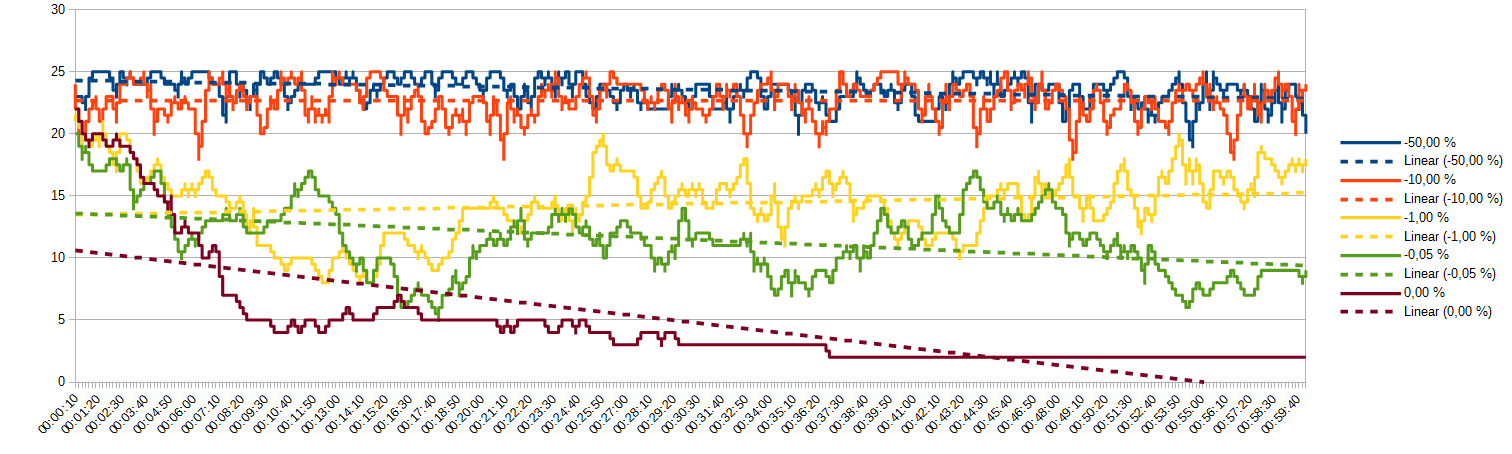
\includegraphics[width=\textwidth, height=\statisticHeight]{graphics/Statistics/FlockGeneral/LocalRange1Speed01FreeWill45NegativeToFlock.png}
	\caption{Entwicklung der Schwärme mit negativem Gruppierungsdrang}
	\label{pic:NegativerGruppierungsdrang}
\end{figure}

Schon ab 1\per negativen Gruppendrangs zeigt die Trendlinie, dass die Gruppen eher dazu neigen sich aufzulösen statt sich neu zu bilden. Der Winkel zur Mitte des eigenen Schwarms kann maximal 180° (in beide Richtungen) groß sein, das heißt der negative freie Wille kann einen Einfluss von maximal 1.8° einnehmen. Trotzdem reicht bereits dieser Einfluss aus um die Roboter zu zu bewegen sich voneinander weg zu bewegen.

Ab einem Wert von 10\per zeigt sich letztlich eine totale Streuung und die Trendlinie bleibt eine Konstante. Die Roboter schaffen es teilweise keinen einzigen Schwarm zu bilden (bzw. nur Schwärme in denen sie selbst als einziger Roboter vertreten sind).

Überraschenderweise zeigt ab einem Wert von 50\per die Trendlinie wieder nach unten und die Roboter scheinen sich erneut zu gruppieren. Der Grund hierführ ist, dass die Roboter beim Ausweichen ihrer Kollegen überschießen und sich so weit in die andere Richtung drehen, dass sie letztlich vom Winkel wieder näher dran sind als vorher. Legt man Wert darauf, dass sich die Roboter verteilen, gilt es also einen passenden Prozentwert einzustellen und diesen nicht zu übertreiben, da man sonst das Gegenteil dessen erreicht was man als Ziel hatte.

\section{Anführer}

Um später Transportaufträge erledigen zu können muss der Schwarm in irgendeiner Form gesteuert werden können. Bei einer direkten Steuerung aller Einheiten des Schwarms wäre das Schwarmverhalten allerdings außer Kraft gesetzt und man hätte schlicht eine Menge gelenkter Roboter. Deswegen wurden Mittel gesucht den Schwarm indirekt zu lenken und fand diese Methode in einem Paper \note{QUELLE} in dem beschrieben wurde wie ein Schwarm über 'eingeweihte Anführer' gesteuert werden kann.

\subsection*{Allgemeines zum Anführer}

Der Anführer bietet eine passive Möglichkeit einen Schwarm zu lenken, ohne dass die normalen Einheiten angepasst werden müssen oder in ihrem Verhalten speziell abweichen müssen. Die normalen Einheiten müssen dadurch nicht wissen, dass sie ein bestimmtes Ziel haben, es muss ihnen nicht einmal bewusst sein, dass sie passiv gesteuert werden. Dadurch, dass er stets in die Richtung des Ziels zeigt pendeln sich die anderen Einheiten des Schwarms aufgrund der Orientierung an den Nachbarn, aber auch aufgrund des Gruppendrangs, ebenfalls auf das Zeil ein. Ein Anführer ist somit eine Art Leuchtturm, der permanent eine Richtung angibt ohne sich von der Umwelt beeinflussen zu lassen und der den anderen Robotern eine Orientierung gibt.
Als Anführer versucht die entsprechende Einheit den Kontakt zu seiner Herde nicht zu verlieren. Damit ist nicht nur der Drang gemeint die Gruppenmitte aufzusuchen. Es ist eine bewusstere Art auf den eigenen Schwarm acht zu geben.

\subsection*{Einbindung des Anführers in ROS}

Der Anführer wurde umgesetzt indem einer normalen Einheit 'plötzlich' bewusst wird, dass sein Schwarm einen bestimmten Ort aufsuchen sollte. Dies wurde umgesetzt indem die Roboter ein neues Topic abonniert haben. Über dieses konnte eine einfache Nachricht mit Koordinaten (x, y) an einen bestimmten Roboter versendet werden. Dieser Roboter wurde zum Anführer und hat versucht seinen Schwarm an die entsprechenden Koordinaten zu lenken. Er lenkt direkt auf das Ziel zu und wartet gegebenenfalls wenn er sich zu weit vom eigenen Schwarm entfernt. Ab einer Entfernung von 75\per der lokalen Reichweite zum Mittelpunkt seiner Herde bleibt er stehen, bis er wieder bei 50\per Entfernung angekommen ist. Anschließend setzt er seinen Weg mormal fort. Wurde der Anführer von seinem Schwarm getrennt setzt er den Weg alleine fort.

\subsection*{Analyse}

Für die Analyse des Anführers wurde der gesamte Schwarm an einer Ecke der Simulation platziert. Die Einheiten waren dabei immer nahe genug beieinander um als einzelner Schwarm angesehen zu werden. Einer der Roboter wurde daraufhin zufällig zum Anführer gewählt und dieser hat versucht seinen Schwarm zum Ziel zu führen.

Auch in dieser Analyse spielt Zufall eine beachtliche Rolle, da der freie Wille der Einheiten darauf ausgelegt ist. Es wurden daher immer 10 Simulationen durchgeführt und aus den mittleren 6 Ergebnissen ein Mittelwert berechnet, um Aureißer möglichst zu ignorieren.

\subsubsection*{Abhängigkeit: Freier Wille}\label{subsubsec:AbhängigkeitFreierWille}

In dieser Statistik wurde geprüft wie sich verschiedene Werte für den freien Willen darauf auswirken, dass der Schwarm zum Ziel geführt werden kann. Über die X-Achse von \autoref{pic:LeaderDependencyFreeWill} hinweg ist die vergangene Wegstrecke in Prozent angegeben, die Y-Achse zeigt die Anzahl der Roboter die im Schwarm des Anführers vorhanden sind.

\paragraph*{Eigenschaften des Schwarms:}
\begin{itemize}
	\item Größe des Schwarms: 25 Roboter
	\item Anzahl der Anführer: 1 Anführer
	\item Lokale Reichweite: 5\per der Größe der Simulation
	\item Geschwindigkeit: 10\per der lokalen Reichweite
	\item Drang zur Gruppierung: 5\per
	\item Freier Wille: Variabel
\end{itemize}

In der \autoref{pic:LeaderDependencyFreeWill} zu sehen, ist dass der Schwarm anfangs immer zusammen blieb. Da die Roboter als gemeinsamer Schwarm zusammen gestartet sind, mussten sie sich nicht erst finden. Wenn der Schwarm in eine andere Richtung lenkte als der Anführer, blieb der Anführer ab einer bestimmten Entfernung stehen und wartete. Zog der Schwarm weiterhin in die Richtung löste er sich irgendwann vom Anführer und dieser zog alleine weiter Richtung Ziel. Durch den relativ hohen Wert von 5\per im Gruppendrang blieb der Schwarm jederzeit zusammen. Wenn sich der Schwarm vom Roboter löste, tat er dies immer im gesamten.

\begin{figure}
	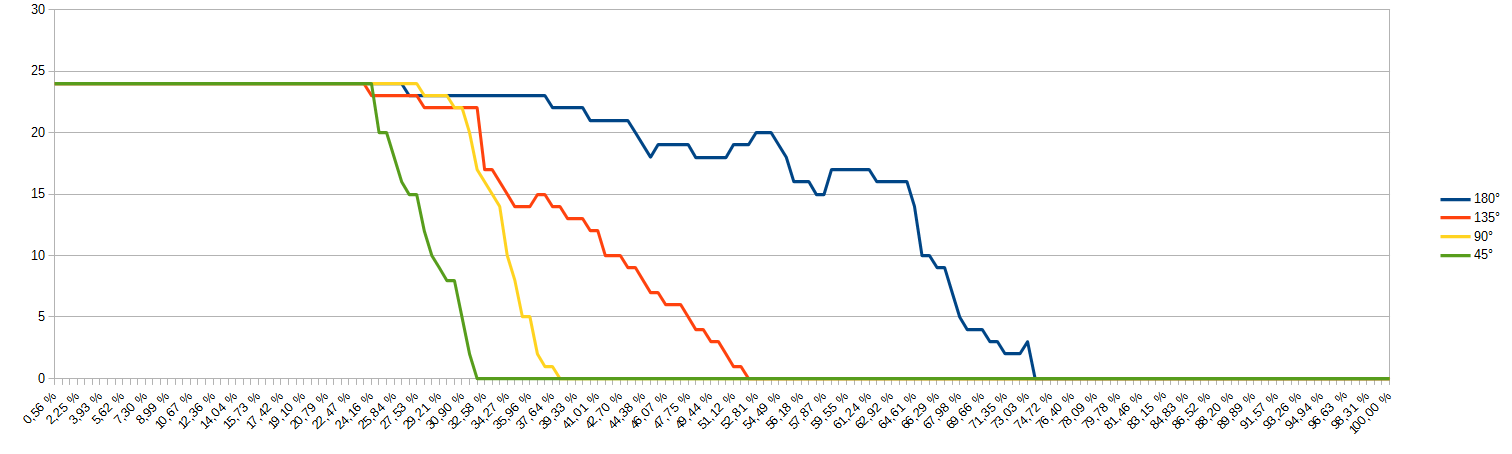
\includegraphics[width=\textwidth, height=\statisticHeight]{graphics/Statistics/Leader/DependencyFreeWill.png}
	\caption{Erfolg eines Anführer ins Abhängigkeit des freien Willens}
	\label{pic:LeaderDependencyFreeWill}
\end{figure}

Je niedriger der Wert im freien Willen war, desto eher löste sich der Schwarm scheinbar von seinem Anführer. Dies ist darauf zurückzufiühren, dass bei einer Gruppengröße von 25 Robotern der Einfluss eines Anführers nur 4.2\per ausmacht und der Schwarm mehr vom Zufall als vom Anführer gelenkt wird. Dass die Roboter mit dem größeren freien Willen letztlich scheinbar länger beim Anführer blieben, ist dem geschuldet, dass die Roboter weniger eng als Schwarm zusammen bleiben und durch die Verteilung der Roboter mehr in der Nähe des Anführers blieben. Die Roboter mit dem geringen freien Willen hingegen blieben mehr zusammen und sind somit 
%
%\subsubsection*{Abhängigkeit: Gruppenzugehörigkeit}
%
%In den folgenden Versuchen wurde geprüft, wie sich die Erfolgsquote des Anführers verändert, wenn statt des freien Willens der Gruppendrang variabel gehalten wird. Über die X-Achse von \autoref{pic:LeaderDependencyToFlockFreeWill90} und \autoref{pic:LeaderDependencyToFlockFreeWill180} hinweg ist die vergangene Wegstrecke in Prozent angegeben, die Y-Achse zeigt die Anzahl der Roboter die im Schwarm des Anführers vorhanden sind.
%
%\paragraph*{Eigenschaften des Schwarms:}
%\begin{itemize}
%	\item Größe des Schwarms: 25 Roboter
%	\item Anzahl der Anführer: 1 Anführer
%	\item Lokale Reichweite: 5\per der Größe der Simulation
%	\item Geschwindigkeit: 10\per der lokalen Reichweite
%	\item Drang zur Gruppierung: Variabel
%	\item Freier Wille: 90° bzw. 180°
%\end{itemize}
%
%Bei einem Gruppendrang von 1\per zeigt sich, ähnlich zu \autoref{subsubsec:AbhängigkeitFreierWille}, dass ein größerer Wert dazu führt, dass die Roboter eher unter sich bleiben und sich weniger streuen. Der Anführer hat mit seinen 4.2\per nicht genug Einfluss um den Schwarm bei sich zu halten und ab einem bestimmten Punkt entschließt sich der Schwarm dazu einen anderen Weg einzunehmen.
%
%\begin{figure}
%	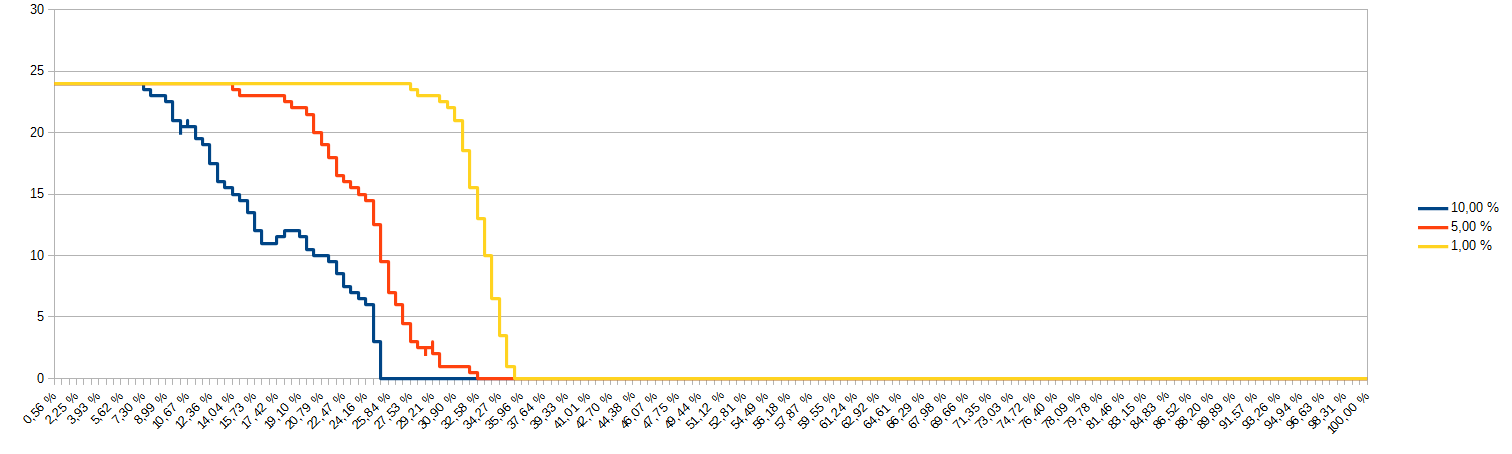
\includegraphics[width=\textwidth, height=\statisticHeight]{graphics/Statistics/Leader/DependencyToFlockFreeWill90_new.png}
%	\caption{Erfolg eines Anführer ins Abhängigkeit der Gruppenzugehörigkeit mit einem freien Willen von 90°}
%	\label{pic:LeaderDependencyToFlockFreeWill90}
%\end{figure}
%
%Auch ähnlich sind die Ergebnisse bei einem freien Willen von 180°. Die Roboter streuen sich mehr und bilden generell mehr Schwärme. Dadurch bleiben automatisch auch mehr Roboter in der Nähe des Anführers, weswegen er es letztlich scheinbar schafft mehr Roboter mit ins Ziel zu führen.
%
%\begin{figure}
%	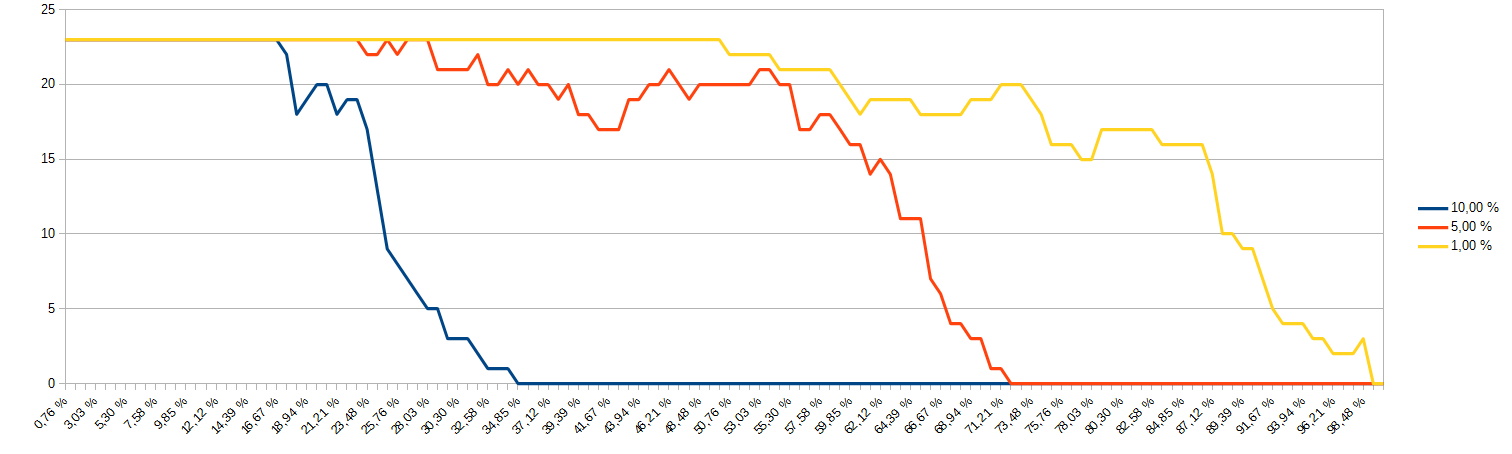
\includegraphics[width=\textwidth, height=\statisticHeight]{graphics/Statistics/Leader/DependencyToFlockFreeWill180_new.png}
%	\caption{Erfolg eines Anführer ins Abhängigkeit der Gruppenzugehörigkeit mit einem freien Willen von 180°}
%	\label{pic:LeaderDependencyToFlockFreeWill180}
%\end{figure}

\subsubsection*{Abhängigkeit: Gruppengröße und -drang}

In den folgenden Statistiken wurde ein Anführer mit steigender Gruppenzahl und unterschiedlichem Gruppendrang gemessen. Über die X-Achse von \autoref{pic:LeaderDependencyFreeWill} hinweg ist der genutzte Gruppendrang angegeben.
Das erste Diagramm zeigt dabei, für wie viel Prozent der Wegstrecke der gesamte Schwarm beisammen gehalten werden konnte.
Das zweite Diagramm zeigt die Größe des Schwarms um den Anführer herum beim erreichen des Ziels.
Das dritte Diagramm zeigt die Anzahl der Wartezeiten die der Anführer hatte. Eine höhere Anzahl an Wartezeiten ist direkt equivalent zu einer längeren Zeit die die Simulation gebraucht hat.

Dabei werden immer 2 Werte gezeigt. 'Mittelwert', der einen einfachen Mittelwert über alle 15 Messwerte anzeigt und 'Median', bei dem der Mittelwert auf die mittleren 10 Messwerte begrenzt wurde um Ausreißer auszusortieren. Da der Anführer selbst immer am Ziel ankommt, wurde er bei den Messwerten abgezogen. Die Anzahl der dargestellten Roboter entspricht also immer denjenigen, die passiv zum Ziel geführt wurden.

\paragraph*{Eigenschaften des Schwarms:}
\begin{itemize}
	\item Größe des Schwarms: Variabel Roboter
	\item Anzahl der Anführer: 1 Anführer
	\item Lokale Reichweite: 5\per der Größe der Simulation
	\item Geschwindigkeit: 10\per der lokalen Reichweite
	\item Drang zur Gruppierung: Variabel
	\item Freier Wille: 90°
\end{itemize}

\begin{figure}
	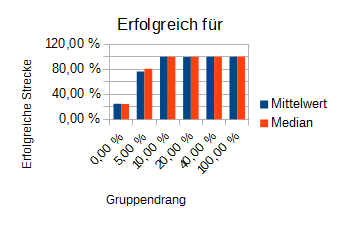
\includegraphics[width=4.9cm, height=4cm]{graphics/Statistics/Leader/FlockSize/5_1.png}
	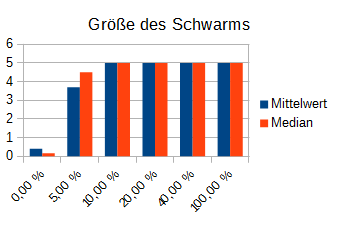
\includegraphics[width=4.9cm, height=4cm]{graphics/Statistics/Leader/FlockSize/5_2.png}
	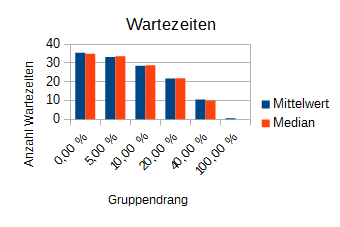
\includegraphics[width=4.9cm, height=4cm]{graphics/Statistics/Leader/FlockSize/5_3.png}
	\caption{Erfolg eines Anführer ins Abhängigkeit der Gruppengröße und des Gruppendrangs mit 5 passiven Robotern}
	\label{pic:LeaderSize5}
\end{figure}

In \autoref{pic:LeaderSize5} zu sehen ist zunächst einmal, dass der Anführer in einer Gruppe mit nur 5 Robotern einen sehr starken Einfluss auf die Gruppe hat. Bereits ohne Gruppendrang gibt es eine Erfolgsquote von über 20\%. Ab 5\per Gruppendrang gibt es schon annähernd 80\per Erfolgsquote und ab 10\per bekommt er seinen Schwarm immer ans Ziel gebracht.

Die Größe des Schwarms zeigt ein sehr ähnliches Bild. Kommen bei 0\per Gruppendrang im Schnitt nur sehr wenige Roboter an, steigert es sich sprunghaft auf 4 Einheiten und ab einem Gruppendrang von 10\per kommen immer alle Roboter an.

Die Wartezeiten sind nicht ganz so konstant, zeigen aber, dass es noch deutliche Unterschiede zwischen den Prozentwerten im Bereich von 10-100\per gibt, auch wenn die beiden vorigen Diagramme dort keine mehr gezeigt haben. Mit einem höheren Gruppendrang sinkt die Anzahl der Wartezeiten immer mehr und bei 100\per gibt es sogar annähernd gar keine mehr.

\begin{figure}
	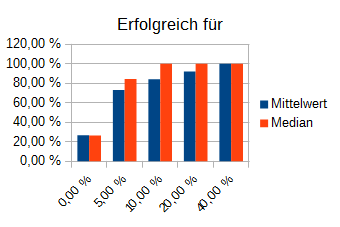
\includegraphics[width=4.9cm, height=4cm]{graphics/Statistics/Leader/FlockSize/10_1.png}
	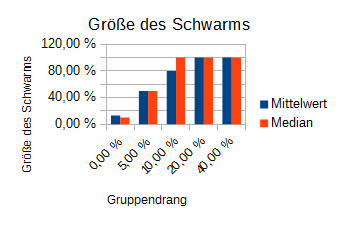
\includegraphics[width=4.9cm, height=4cm]{graphics/Statistics/Leader/FlockSize/10_2.png}
	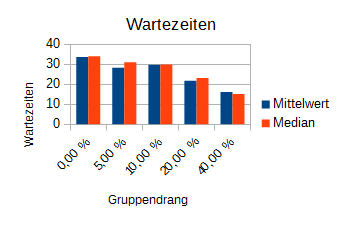
\includegraphics[width=4.9cm, height=4cm]{graphics/Statistics/Leader/FlockSize/10_3.png}
	\caption{Erfolg eines Anführer ins Abhängigkeit der Gruppengröße und des Gruppendrangs mit 10 passiven Robotern}
	\label{pic:LeaderSize10}
\end{figure}

Die Diagramme in \autoref{pic:LeaderSize10} zeigen, dass der Einfluss des Anführers mit 5 Robotern mehr schon deutlich nachlässt. Konnten vorher scon ab 10\per Gruppendrang beste Ergebnisse erziehlt werden, zeigt der Durchschnitt nun deutlich niedrigere Werte. Dies bedeutet vor allem dass die Fehlerquote zunahm und die 10 mittleren Ergebnisse nun ebenfalls höhere Schwankungen aufweisen. Nur bei 40\per sieht man noch einen vollen Erfolg über alle Messwerte hinweg.

Die Größe des Schwarms ist von ähnlichen Rückschlägen betroffen. Bei 0\per Gruppendrang schafft es nur jeder zehnte Roboter ins Ziel, fast der gleiche Wert wie bei 5 passiven Robotern. Bei 10\per Gruppendrang schafft es der Median auf einen vollen Erfolg, der Mittelwert hingegen erst ab 20\%.

Die Wartezeiten zeigen hingegen nicht unbedingt den gleichen Trend. Sie sind zwar allgemein stiegen, der Trend ist aber nicht mehr so steil wie in der Statistik mit 5 passiven Robotern. Steigen beide Diagramme bei ca. 30 Wartezeiten ein, ist nun auch bei 40\per Gruppendrang eine deutlich höhere Wartezeit zu sehen.

\begin{figure}
	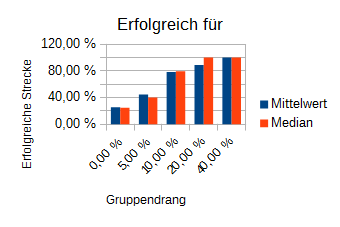
\includegraphics[width=4.9cm, height=4cm]{graphics/Statistics/Leader/FlockSize/15_1.png}
	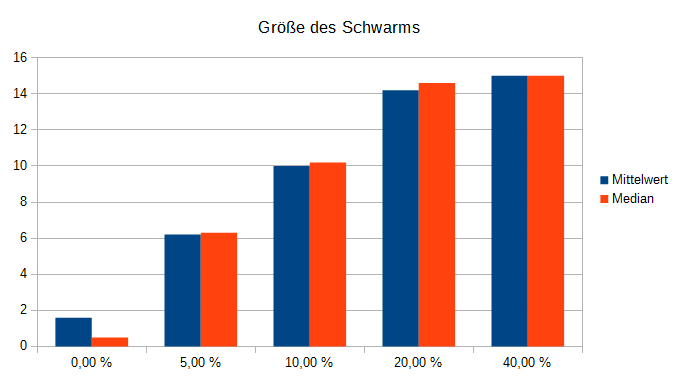
\includegraphics[width=4.9cm, height=4cm]{graphics/Statistics/Leader/FlockSize/15_2.png}
	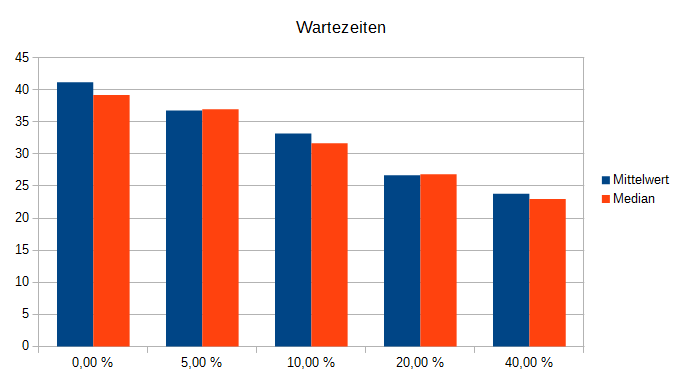
\includegraphics[width=4.9cm, height=4cm]{graphics/Statistics/Leader/FlockSize/15_3.png}
	\caption{Erfolg eines Anführer ins Abhängigkeit der Gruppengröße und des Gruppendrangs mit 15 passiven Robotern}
	\label{pic:LeaderSize15}
\end{figure}

In \autoref{pic:LeaderSize15} nimmt der allgemeine Trend weiter seinen Lauf. Die Erfolgsquote für die Werte unter 40\per nehmen immer weiter ab, wenn auch die 40\per selbst noch einen vollen Erfolg vorweisen kann.

Es kommen auch weniger Roboter insgesamt im Ziel an, wenn die Gesamtzahl der ankommenden Roboter auch bei 20\per Gruppendrang noch recht hoch ist. Bei 40\per Gruppendrang ist nach wie vor ein voller Ausschlag zu sehen.

Auch die Wartezeiten zeigen den selben Trend wie zuvor. Sie starten recht hoch, der Trend bleibt aber flacher als bei den Messungen mit 5 passiven Robotern weniger.

\begin{figure}
	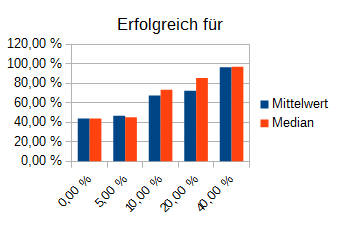
\includegraphics[width=4.9cm, height=4cm]{graphics/Statistics/Leader/FlockSize/20_1.png}
	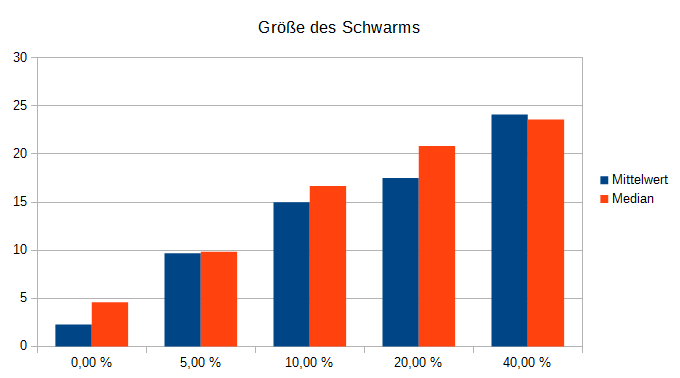
\includegraphics[width=4.9cm, height=4cm]{graphics/Statistics/Leader/FlockSize/20_2.png}
	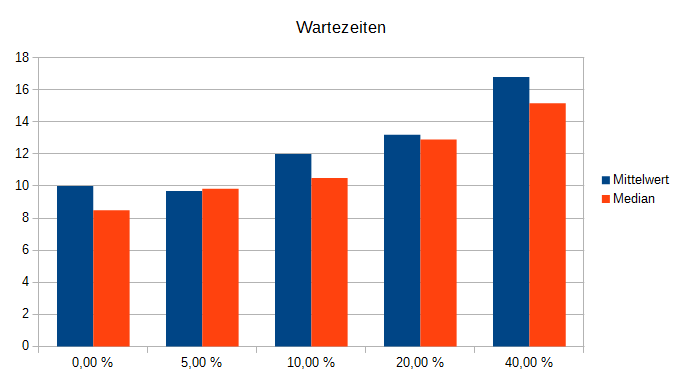
\includegraphics[width=4.9cm, height=4cm]{graphics/Statistics/Leader/FlockSize/20_3.png}
	\caption{Erfolg eines Anführer ins Abhängigkeit der Gruppengröße und des Gruppendrangs mit 20 passiven Robotern}
	\label{pic:LeaderSize20}
\end{figure}

Ab einer passiven Anzahl von 20 Robotern zeigt sich in \autoref{pic:LeaderSize20} erstmals der Trend, dass die Wartezeiten zunehmen, wenn der Gruppendrang größer wird. Ein genauerer Blick auf das Diagram zeigt jedoch auch, dass die Wartezeiten allgemein sehr viel niedriger sind als in den Messungen mit weniger Robotern. Dies ist vor allem darauf zurückzuführen, dass der Anfüher ab einer Zahl von 20 passiven Robotern einen Schwarm viel schneller vollständig verliert und es keine Wartezeiten mehr gibt, weil er schneller dazu übergeht das Ziel alleine aufzusuchen. Auch die anderen beiden Diagramme zeigen nun bei 40\per Gruppendrang keinen vollen Erfolg mehr.

\begin{figure}
	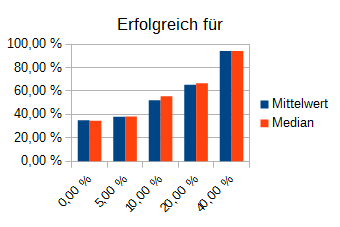
\includegraphics[width=4.9cm, height=4cm]{graphics/Statistics/Leader/FlockSize/25_1.png}
	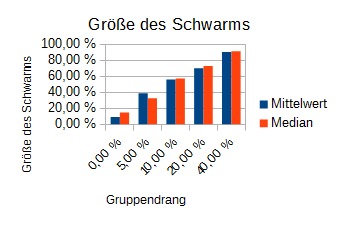
\includegraphics[width=4.9cm, height=4cm]{graphics/Statistics/Leader/FlockSize/25_2.png}
	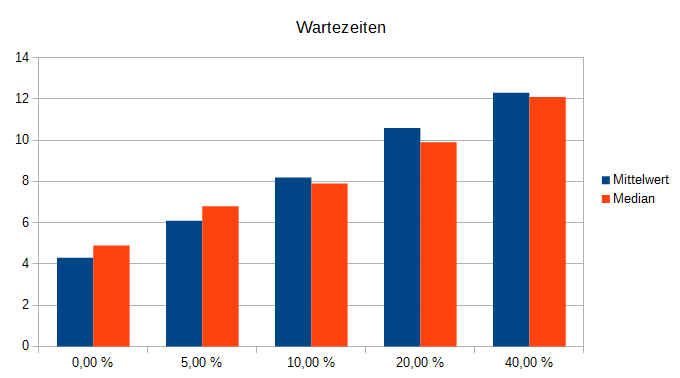
\includegraphics[width=4.9cm, height=4cm]{graphics/Statistics/Leader/FlockSize/25_3.png}
	\caption{Erfolg eines Anführer ins Abhängigkeit der Gruppengröße und des Gruppendrangs mit 25 passiven Robotern}
	\label{pic:LeaderSize25}
\end{figure}

In den letzten Diagrammen (\autoref{pic:LeaderSize25}) ist letztlich zu sehen dass sich der allgemeine Trend weiter fort führt. Die Wartezeiten sinken noch deutlicher, weil der Anführer seinen Schwarm immer früher verliert. Die erfolgreiche Strecke nimmt genau wie die Anzahl der Roboter die im Ziel ankommen immer mehr ab. Nur bei 40\per Gruppendrang bleiben die Werte noch immer recht hoch.


\section{Transport von Waren mit Hilfe eines Schwarms}

Das letztliche Ziel dieser Arbeit ist es zu prüfen, ob es möglich, und sinnvoll, ist Gegenstände mit Hilfe eines autonomen Schwarms zu transportieren. Dazu musste der Schwarm nun dazu gebracht werden Waren zu bewegen ohne die einzelnen Roboter zu sehr zu beeinflussen. Da generell die Roboter nicht zentral gesteuert werden sollen und auch die Logik möglichst simple bleiben soll, sollte das Programm der einzelnen Einheiten möglichst wenig verändert werden und der 'natürliche' Trieb der Einheiten genutzt werden.

\subsection*{Erteilen von Aufträgen}

Eine der ersten Dinge im Ablauf eines Transports ist die Erteilung des Auftrags. Dazu wurde ein neuer Nachrichten-Typ Namens 'MissionNew' im ROS-Netzwerk eingeführt der die folgenden Felder hat:

\begin{lstlisting}[frame=L]
uint8 robot_index_from
uint8 robot_index_to

uint8 leader_number
uint8 mission_id

float32 object_position_x
float32 object_position_y

float32 object_size_x
float32 object_size_y

float32 target_x
float32 target_y
\end{lstlisting}

Der Nachrichten-Typ definiert eine Spanne von Robotern die den Auftrag ausführen sollen. Diese werden mit ihren IDs angesprochen. Das Intervall der IDs ist, gemäß Programmierstandards, als halboffenes Intervall definiert: [robot\_index\_from, robot\_index\_to[.
leader\_number gibt die Anzahl der Leader an die verwendet werden sollen und mission\_id gibt dem derzeitigen Auftrag eine fixe ID um diesen und zugehörige Dinge genau identifizieren und verbinden zu können.
Mit object\_position\_x/-\_y ist die Startposition des zu transportierenden Objektes angegeben. Zusammen mit object\_size\_x/-\_y, welche die Ausmaße des Objektes angeben. Die Position des Objekts ist als Mitte des Objekts definiert.
target\_x/-\_y gibt die letztliche Position an die das Objekt einnehmen soll.

Der Auftrag wird von außen an das Topic 'flock/mission/new' gesendet. Der Ersteller des Auftrags muss keine ROS-Node sein, auch wenn dies verschiedene Vorteile hätte. Dadurch das ROS-Topics auch über das Terminal engesprochen werden können, ist das Senden der Nachrichten auch über jedes andere Programm möglich. Das Topic für die neuen Missionen wird von jedem aktiven Roboter abonniert. Entsprechend nimmt jeder Roboter Notiz von diesem Auftrag, auch wenn er nicht direkt mit seiner ID angesprochen wird.

\subsection*{Von Gefahrenzonen zu Sicherheitszonen}

Um die betreffenden Roboter in die Zone zu senden, auf der ihnen später das Transportobjekt aufgesetzt wird, wird ein Mechanismus verwendet der bereits vorher Einzug in das ROS-System hielt: Gefahrenzonen. Diese wurden leicht angepasst um sie invertieren zu können und somit aus einer Gefahrenzone eine Sicherheitszone zu machen. Ist ein Bereich als Sicherheitszone definiert, ist jeder andere Bereich automatisch eine Gefahrenzone.
Dieser Mechanismus birgt nur eine kleine Änderung im System, schafft es aber Roboter in einen bestimmten Bereich zu locken ohne sie aktiv steuern zu mpsse, indem einfach ihr 'natürlicher' Trieb verwendet wird, von Gefahren zu flüchten.

Wird ein Auftrag erteilt, so nehmen die Roboter die dem Auftrag zugeteilt sind, eine neue Sicherheitszone auf, die den Ausmaßen und der Position des Transportobjekts am Aufnahmeort entsprechen. Roboter die nicht dem Transport zugeteilt wurden, werden diese neue Zone als Gefahrenzone auffassen und versuchen sich diesem Gebiet fernzuhalten.

Ein Objekt kann grundsätzlich aus verschiedenen Geometrien zusammengesetzt werden. Dadurch ist es möglich nicht nur Objekte zu transportieren die eine einfache Form wie Rechtecke oder Kreise haben, sondern verschiedene Rechtecke können dann zu einem 'L' oder 'U' zusammengesetzt werden.

\begin{wrapfigure}{r}{\pictureWidth}
	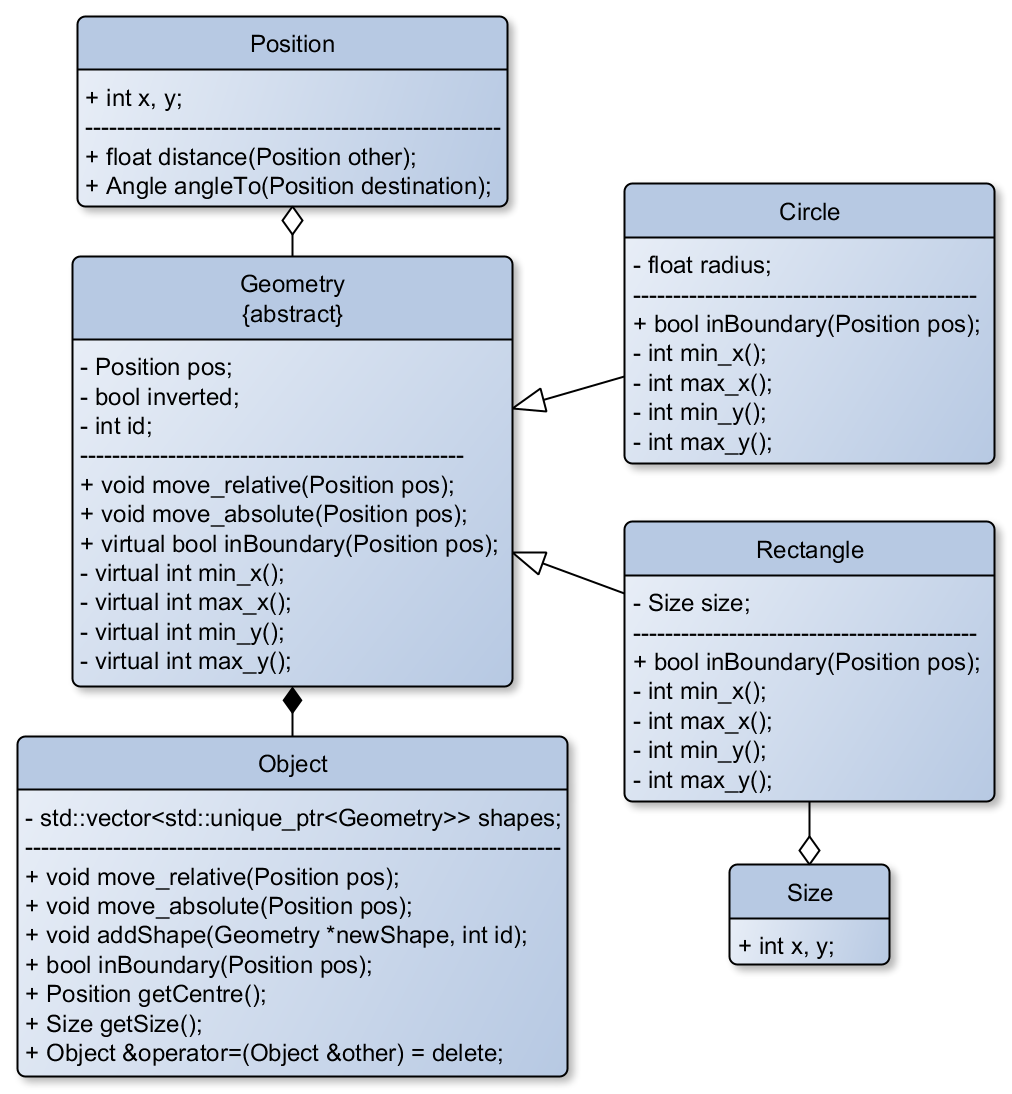
\includegraphics[width=\pictureWidth,keepaspectratio]{graphics/Klassendiagramme/KlassendiagrammObject.png}
	\caption{Die Klassenhierarchie des Objekt-Systems}
	\label{pic:KlassendiagrammObject}
\end{wrapfigure}

\paragraph*{Implementierung}
Die Klassenhierarchie ist wie in \autoref{pic:KlassendiagrammObject} dargestellt. Die Implementierung eines Objekts ist als Sammelklasse definiert, die verschiedene Geometrien unter sich vereint. Die Geometrien haben eine Hauptklasse von der sie sich ableiten. Die abgeleiteten Klassen müssen letztlich nur noch definieren, wann etwas innerhalb ihrer Fläche ist und was ihre Ausmaße im zweidimensionalen Raum sind. Wird ein Objekt auf eventuelle Kollisionen abgefragt, muss dieses letztlich nur noch über die inneliegenden Geometrien iterieren und sobald eine Kollision statt fand ist das Gesamtergebnis ebenfalls eine Kollision.

\subsection*{Füllen eines Raums}

Wird eine Sicherheitszone definiert, versuchen die Roboter, die sich in der Gefahrenzone befinden, auf möglichst schnellstem Wege die Sicherheitszone zu betreten. Dazu wird das Zentrum der Sicherheitszone ins Ziel genommen und (ohne mit anderen Robotern zu kollidieren) der direkte Weg darauf zu genommen. Dabei kann es dann allerdings vorkommen, dass eine komplexere Form nicht vernünftig gefüllt werden kann, oder dies sehr lange dauert. Da ein eintreffender Roboter so lange auf den Mittelpunkt zufahren würde, bis die Roboter darin sich genug verteilt haben um genug Platz für den neuen Roboter zu schaffen.

Ein Algorithmus wie man es schafft mit Roboter einen definierten Raum zu füllen lässt sich in (\note{HIER; QUELLE}) finden. Dieser Algorithmus lässt sich aufgrund anderer Fähigkeiten bei den Robotern nicht und dem gewünschten Schwarmverhalten nicht vollständig nachbilden. Eine andere, bereits implementierte Fähigkeit, lässt sich dagegen gut nutzen um den Algorithmus annähernd nachzubauen: Ausweichen.

\begin{wrapfigure}{r}{\pictureWidth}
	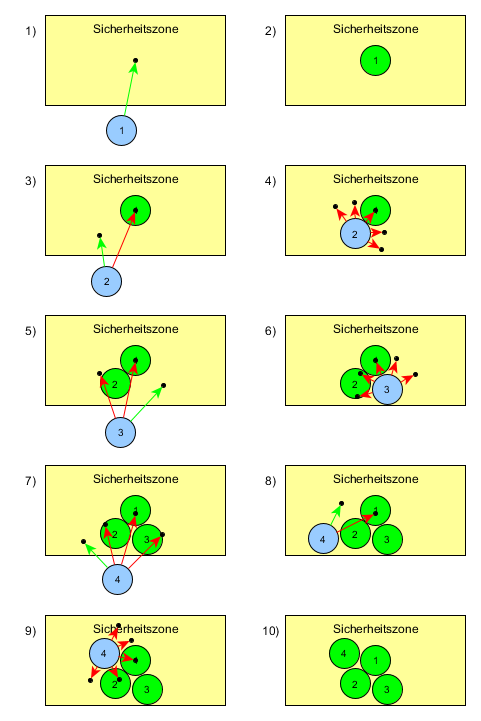
\includegraphics[width=\pictureWidth,keepaspectratio]{graphics/AlgorithmusAusweichenTransport.png}
	\caption{Roboter füllen das Transportobjekt}
	\label{pic:AlgorithmusAusweichenObjekt}
\end{wrapfigure}

Betritt ein Roboter die Sicherheitszone des Transport-Objekts, reduziert dieser seine Geschwindigkeit und fährt langsam weiter auf den Mittelpunkt zu. Neu ankommende Roboter werden durch die vorderen, viel langsameren Roboter zum Ausweichen gezwungen, was letztlich dazu führt, dass die Roboter sich seitlich verteilen, aber langfristig den Nachfolgern Platz machen. Ist ein Roboter nahe genug am Mittelpunkt angekommen oder findet in einem Umkreis von [-90°, 90°] keinen Platz mehr der näher am Mittelpunkt ist als der aktuelle, bleibt er stehen. Roboter die stehen bleiben senden den anderen Robotern ihres Schwarms ein entsprechendes Signal dass sie bereit sind. Haben alle Roboter erkannt dass die anderen bereit sind, ist die Phase des Eintreffens am Abnahmepunkt abgeschlossen.

Von hier an braucht es ein Event dass den Robotern zeigt dass sie mit dem Transportobjekt Richtung Ziel losfahren können. Möglich wäre eine Zeitsteuerung für streng automatisierte Prozesse. Aber auch interne Signale über ROS sind möglich. Durch die ID die jeder Auftrag hat, wäre eine einfache Nachricht '[TransportID\#][Losfahren]' bereits zielführend.

\paragraph*{Der Algorithmus am Beispiel}
\autoref{pic:AlgorithmusAusweichenObjekt} zeigt den Algorithmus anhand eines Beispiels mit 4 Robotern.

Der erste Roboter versucht zur Mitte des Objekts zu gelangen und findet sofort Zugang zum Objekt. Er reduziert seine Geschwindkeit und platziert sich langsam im Mittelpunkt des Objektes. Da seine Nähe zum Mittelpunkt klein genug ist, bleibt er letztlich stehen.

Der nächste Roboter kommt, wird allerdings von seinem Vorgänger leicht blockiert. Das führt dazu dass dieser versucht nach links auszuweichen und damit Erfolg hat. Er betritt die Zone, findet aber keinen besseren Ort und bleibt daraufhin stehen.

Der dritte Roboter wird ebenfalls von seinen Vorgängern blockiert, findet aber rechts eine Stelle. Nachdem er diese eingenommen hat findet auch er keine bessere Stelle und bleibt ebenfalls stehen.

Der vierte Roboter findet zunächst links eine Stelle und betritt daraufhin die Zone. Er verlangsamt seine Bewegung und sucht nun nach Stellen die ihn ohne Kollisionen näher zu seinem Ziel führen, wobei er einmal Roboter\#2 umkreist. In der Lücke zwischen Roboter\#2 und Roboter\#1 findet er die beste Stelle und bleibt dort anschließend stehen. Der Algorithmus für diese 4 Roboter ist damit abgeschlossen. Sie stehen alle in der Fläche des Transportobjektes und stehen still, bereit die Lieferung entgegen zu nehmen.

\subsection*{Der Transport}

Um den Transport selbst zu realisieren bedient man sich der Hilfe der Anführer. Diese richten sich dynamisch nach dem Winkel aus, den das Transportobjekt zum Ziel hat, wie \autoref{pic:AlgorithmusTransport} zeigt. Danach fangen sie an sich langsam in die Richtung zu bewegen in die sie sich ausgerichtet haben. Die anderen Roboter werden sich aufgrund des Gruppenverhaltens ebenfalls mehr oder weniger nach ihren Anführern ausrichten und das Objekt so langsam Richtung Ziel bewegen.

\begin{wrapfigure}{r}{\pictureWidth}
	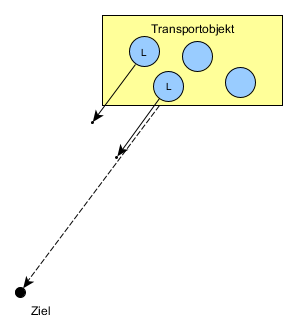
\includegraphics[width=\pictureWidth,keepaspectratio]{graphics/AlgorithmusTransport.png}
	\caption{Der Transport des Objekts}
	\label{pic:AlgorithmusTransport}
\end{wrapfigure}

\subsubsection*{Einhalten der Richtung hat Priorität}
Kann ein Anführer keine normale Bewegung ausführen, weil er sonst mit einem anderen Roboter kollidieren würde, darf er nicht versuchen auszuweichen, da dies sonst die Ausrichtung der passiven Roboter negativ beeinflussen könnte. Stattdessen drosselt er zunächst sein Bewegungstempo oder bleibt, falls notwendig, ganz stehen. Die richtige Richtung beizuhalten ist wichtig, da sich passive Roboter nicht unmittelbar nach ihren Anführern ausrichten. Gerade wenn es zahlenmäßig wenige Anführer im Vergleich zu passiven Robotern sind, kann es einige Zeit dauern, bis die Einheiten so weit beeinflusst wurden, dass sie in die gewünschte Richtung zeigen. Dreht sich ein Anführer in die verkehrte Richtung, vielleicht sogar in die entgegengesetzte, kann dies zu einer Kettenreaktion führen die alle Roboter betrifft und zusätzlich das Transportobjekt stark vom Weg abbringen.

\subsubsection*{Abschluss des Transports}






